\begin{document}

The previously constructed Optical Uplink transmitter modules is made up of CMOS astable multivibrator circuit which provides the driving signal for the LED. A schematic of the transmitter is shown below in Figure \ref{fig:finalexperimentalschem}

\begin{figure}[H]
	\centering
	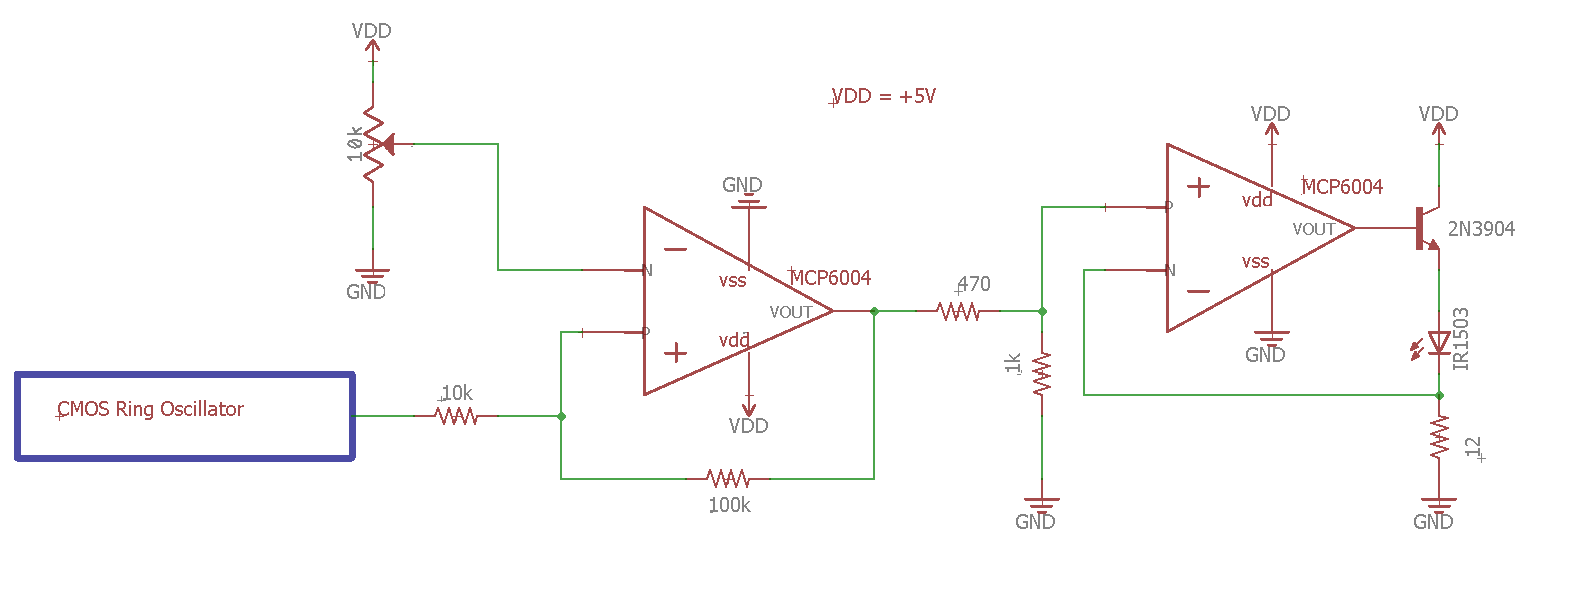
\includegraphics[width=0.7\linewidth]{Preliminary_results/FINAlexperimentalSchem}
	\caption[Circuit schematic of transmitter]
	\label{fig:finalexperimentalschem}
\end{figure}

The astable multivibrator is constructed on a signal CD4007 MOS DIP, which consists of three CMOS circuits. The waveform is then conditioned with a Schmitt trigger and then passed through a amplifier, both constructed on an MCP6004 quad-op-amp. This, in turn, drives an 2N3904 BJT, which controls the current through the IR1503 LED. The resulting current is seen in Figure \ref{fig:expcurrentlab4}.

\begin{figure}[H]
	\centering
	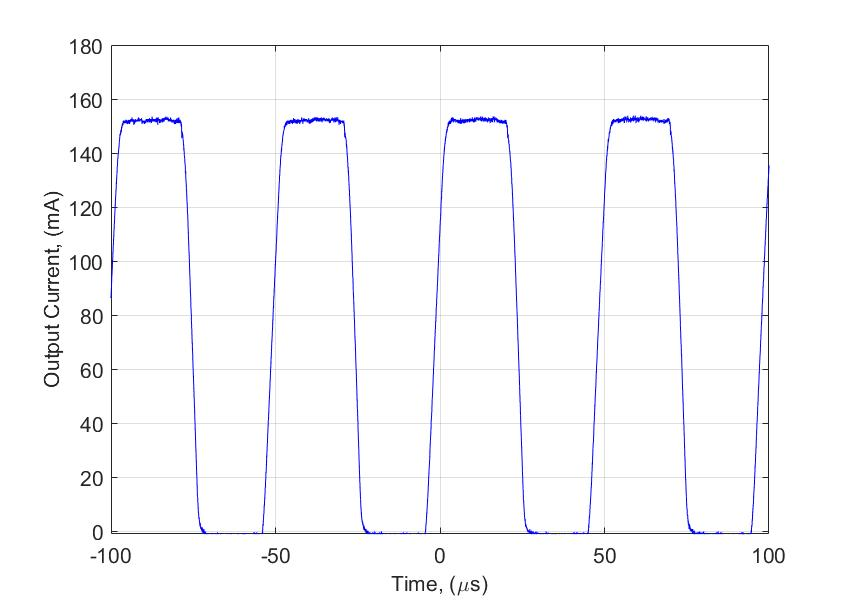
\includegraphics[width=0.7\linewidth]{Preliminary_results/expcurrentlab4}
	\caption[Current through LED]
	\label{fig:expcurrentlab4}
\end{figure}


	
\end{document}